
\documentclass[11pt,a4paper]{article}
\usepackage[utf8]{inputenc}
\usepackage[T1]{fontenc}
\usepackage[brazil]{babel}
\usepackage{amsmath, amssymb}
\usepackage{graphicx}
\usepackage{booktabs}
\usepackage{hyperref}
\usepackage{geometry}
\usepackage{xcolor}
\usepackage{listings}
\usepackage{caption}
\geometry{margin=2.3cm}
\lstset{
  basicstyle=\ttfamily\footnotesize,
  breaklines=true,
  frame=single,
  numbers=left,
  numberstyle=\tiny,
  tabsize=2,
  showstringspaces=false
}

\begin{document}
\begin{titlepage}
    \centering
    \vspace*{0.5cm}
    
\includegraphics[width=0.35\textwidth]{EP.jpg}\par\vspace{1cm}
    {\scshape\LARGE Escola Politécnica da Universidade de São Paulo \par}
    \vspace{1.2cm}
    {\scshape\Large PTC5725 -- Introdução aos Métodos Espectrais \par}
    \vspace{2.0cm}
    {\huge\bfseries Relatório: Segunda Lista de Exercícios\par}
    \vspace{2.0cm}
    {\Large Renan de Luca Avila\par}
    \vfill
    São Paulo, \today
\end{titlepage}

\section*{Resumo}
Este documento contempla os quatro exercícios da Aula 02 e duas extensões (Ortogonalidade e Performance). Para cada exercício: Preliminares Teóricos, Enunciado, Entendimento e Raciocínio, Código, Figuras/Tabelas e Conclusões numéricas. \textbf{Adicionalmente, o documento contempla duas extensões de exercícios voluntárias, uma para estudo visual de ortogonalidade de funções e outra para estudo de benchmark de performance entre Python e Julia.}
\paragraph{Apêndice} Alguns códigos reutilizam funções, que foram concentradas em um arquivo chamado utils.py, que está contido no apêndice A. 

\section{Exercício 1 --- Interpolação (Lagrange vs Baricentrica)}

\subsection*{Enunciado}
Interpolar $f(x)=10^3\sin(\pi x)$ com $n=21$ nós e avaliar em 501 pontos equidistantes; comparar Lagrange vs baricêntrica.

\subsection*{Preliminares Teóricos}
Dados os nós $\{x_j\}_{j=0}^{n}$ e $f_j=f(x_j)$,
\begin{equation}
L(x)=\sum_{j=0}^n \ell_j(x)\,f_j,\qquad
\ell_j(x)=\prod_{\substack{k=0\\k\neq j}}^n \frac{x-x_k}{x_j-x_k}.
\end{equation}
Forma baricêntrica com $w_j=\big(\prod_{k\neq j}(x_j-x_k)\big)^{-1}$:
\begin{equation}
p(x)=\frac{\sum_{j=0}^{n}\frac{w_j f_j}{x-x_j}}{\sum_{j=0}^{n}\frac{w_j}{x-x_j}}.
\end{equation}
Usamos os nós de Chebyshev-Lobatto $x_i=\cos(i\pi/n)$.

\subsection*{Entendimento e Raciocínio}
A forma baricêntrica reordena Lagrange para maior estabilidade numérica quando $x\approx x_j$. Avaliamos erros na malha fina; veja Tabela~\ref{tab:ex1}, Fig ~\ref{fig:ex1_interp} e Fig.~\ref{fig:ex1_err}.

\subsection*{Código}
\lstinputlisting{code/ex1_interpolacao.py}

\subsection*{Figuras}
\begin{figure}[h!]\centering
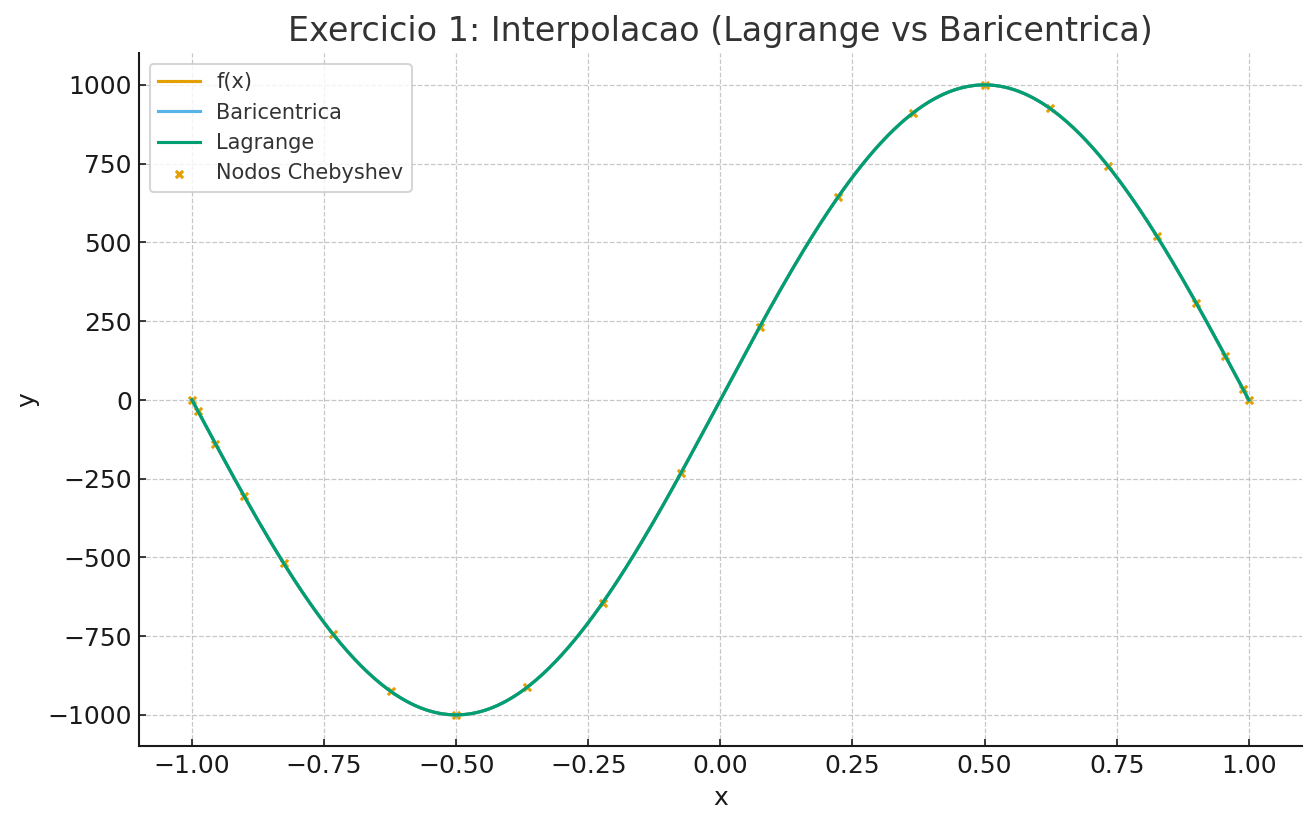
\includegraphics[width=0.85\linewidth]{figures/ex1_interp.png}
\caption{Interpolação em nós de Chebyshev: Lagrange vs Baricentrica.}
\label{fig:ex1_interp}
\end{figure}
\begin{figure}[h!]\centering
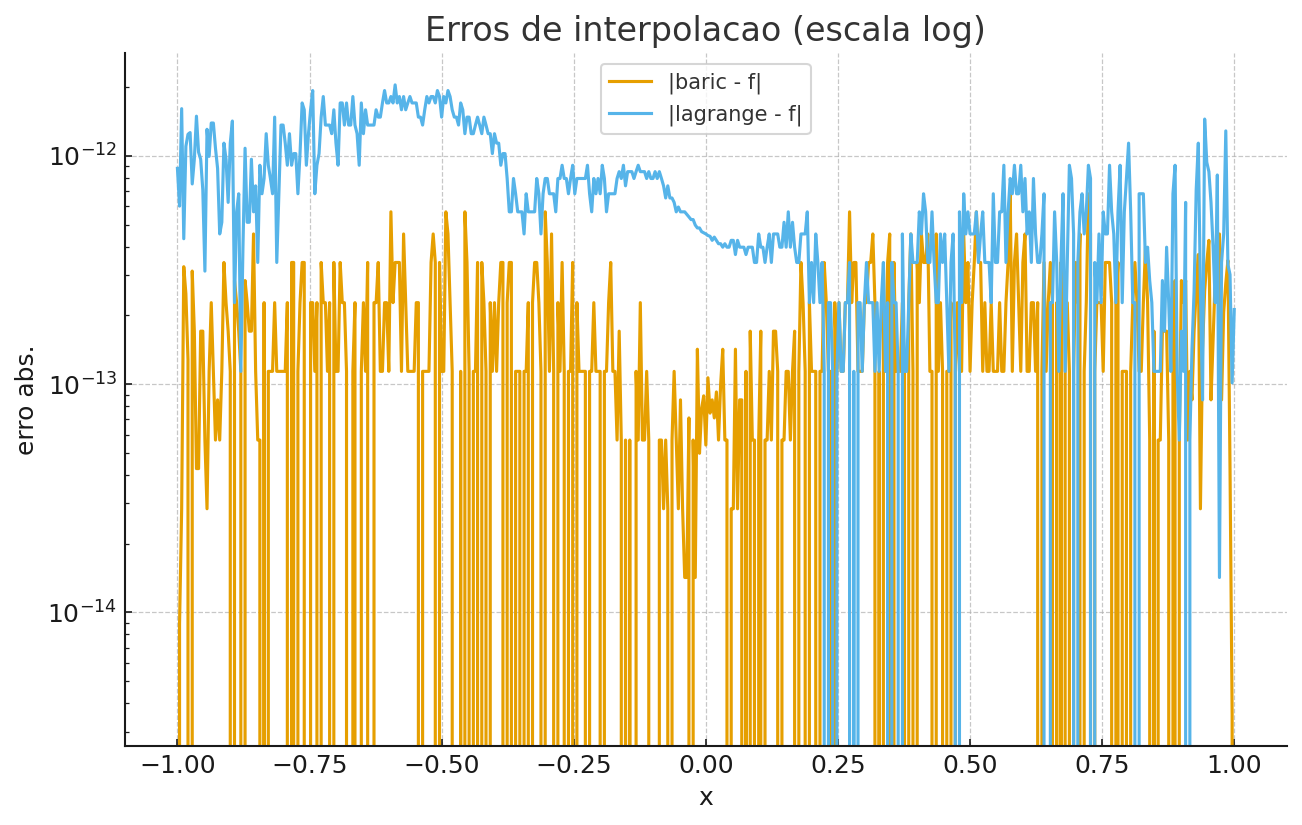
\includegraphics[width=0.75\linewidth]{figures/ex1_errors.png}
\caption{Erros absolutos (escala log).}
\label{fig:ex1_err}
\end{figure}

\subsection*{Tabela e Conclusão}
\begin{table}[h!]\centering
\caption{Exercício 1: erros absolutos em malha de 501 pontos.}
\label{tab:ex1}
\begin{tabular}{lrr}
\toprule
Métrica & Baricêntrica & Lagrange \\
\midrule
$\max|p-f|$ & 6.821e-13 & 2.046e-12 \\
$\mathrm{mean}|p-f|$ & 1.610e-13 & 7.213e-13 \\
\bottomrule
\end{tabular}
\end{table}

Embora as curvas de Lagrange e baricêntrica pareçam idênticas na Fig.~\ref{fig:ex1_interp}, 
seus erros numéricos diferem. Ambas expressam o mesmo polinômio interpolador, 
mas a forma baricêntrica reescreve sua avaliação de modo mais estável, evitando cancelamentos 
numéricos quando $x \approx x_j$. Assim, a interpolação baricêntrica mantém a precisão de ponto 
flutuante e apresenta erros médios e máximos menores (Tabela~\ref{tab:ex1}, 
Fig.~\ref{fig:ex1_err}).

\section{Exercício 2 --- Matriz de Base de Chebyshev}

\subsection*{Enunciado}
Construir, analisar e utilizar a \emph{matriz de base de Chebyshev} $B$ em nós de Lobatto, estabelecendo a transformação discreta entre valores amostrados de uma função e seus coeficientes na base $\{T_j\}_{j=0}^n$, bem como a transformação inversa. Avaliar propriedades numéricas (condicionamento) e validar a exatidão para polinômios de grau $\le n$.

\subsection*{Preliminares Teóricos}

Com $T_n(\cos\theta)=\cos(n\theta)$, a base discreta em $x_i=-\cos(i\pi/n)$ e $B_{i+1,j+1}=T_j(x_i)$.

\begin{itemize}
  \item $T_n(x)$ --- polinômio de Chebyshev de primeira espécie de grau $n$, definido por $T_n(\cos\theta) = \cos(n\theta)$.
  \item $x$ --- variável independente contínua no intervalo $[-1, 1]$.
  \item $\theta$ --- variável angular associada a $x$ por meio da transformação $x = \cos\theta$, com $\theta \in [0, \pi]$.
  \item $n, m$ --- índices inteiros não negativos que representam os graus dos polinômios de Chebyshev.
  \item $w(x)$ --- função de peso usada na relação de ortogonalidade, dada por $w(x) = (1 - x^2)^{-1/2}$.
  \item $\langle T_n, T_m \rangle$ --- produto interno definido como $\displaystyle \int_{-1}^1 T_n(x)T_m(x)w(x)\,dx$.
  \item $B$ --- matriz de base de Chebyshev de ordem $(n{+}1)\times(n{+}1)$, cujos elementos são $B_{i+1,j+1} = T_j(x_i)$.
  \item $x_i$ --- nós discretos de Chebyshev (ou nós de Lobatto), dados por $x_i = -\cos(i\pi/n)$, $i=0,1,\dots,n$.
  \item $i, j$ --- índices discretos que percorrem, respectivamente, as linhas (nós) e colunas (graus) da matriz $B$.
\end{itemize}



\subsection*{Entendimento e Raciocínio}
Neste exercício, buscamos compreender como a \emph{matriz de base de Chebyshev} $B$ representa a relação entre o espaço físico, composto pelos valores de uma função $f(x)$ avaliados nos nós de Lobatto, e o espaço espectral, composto pelos coeficientes da expansão de Chebyshev. 
Cada linha de $B$ contém as avaliações dos polinômios $T_j(x)$ nos nós $x_i = -\cos(i\pi/n)$, de modo que
\[
B_{i+1,j+1} = T_j(x_i) = \cos(j\,\arccos(x_i)).
\]
O código implementa essa definição de forma direta: calcula primeiro os nós $x_i$ e seus ângulos $\theta_i = \arccos(x_i)$, e então preenche a matriz $B$ coluna a coluna usando a relação $T_j(x_i)=\cos(j\theta_i)$. 
Os resultados são exportados em formato CSV e visualizados por meio de um \emph{heatmap} (Fig.~\ref{fig:ex2_B}), em que as colunas representam os polinômios de Chebyshev de diferentes graus — percebe-se que, conforme o índice $j$ aumenta, as oscilações se tornam mais rápidas, refletindo a frequência crescente dos termos $\cos(j\theta)$.

\paragraph{Extra:} Para avaliar a \emph{estabilidade numérica} dessa base, utilizamos a \textbf{decomposição em valores singulares} (SVD, do inglês \emph{Singular Value Decomposition}). 
A SVD fatoriza a matriz $B$ como
\[
B = U\,\Sigma\,V^{\top},
\]
em que $U$ e $V$ são matrizes ortogonais e $\Sigma$ é diagonal contendo os \emph{valores singulares} $\sigma_1 \ge \sigma_2 \ge \dots \ge \sigma_{n+1} > 0$. 
O \emph{número de condição} de $B$ é então definido como
\[
\kappa_2(B) = \frac{\sigma_{\max}(B)}{\sigma_{\min}(B)} = \frac{\sigma_1}{\sigma_{n+1}},
\]
o que fornece uma medida de sensibilidade numérica: quanto maior $\kappa_2$, maior a amplificação de erros de arredondamento em operações envolvendo $B$.

A Tabela~\ref{tab:ex2} apresenta os principais resultados: o menor e o maior valor singular ($\sigma_{\min}$ e $\sigma_{\max}$), o número de condição $\kappa_2(B)$ e o valor médio absoluto dos elementos de $B$. 
Os valores obtidos indicam que $\sigma_{\min}$ permanece significativamente diferente de zero e que o número de condição $\kappa_2(B)$ está dentro de uma faixa moderada, assegurando que a base de Chebyshev é numericamente estável para $n=16$.


\subsection*{Código}
\lstinputlisting{code/ex2_base_chebyshev.py}

\begin{figure}[h!]\centering
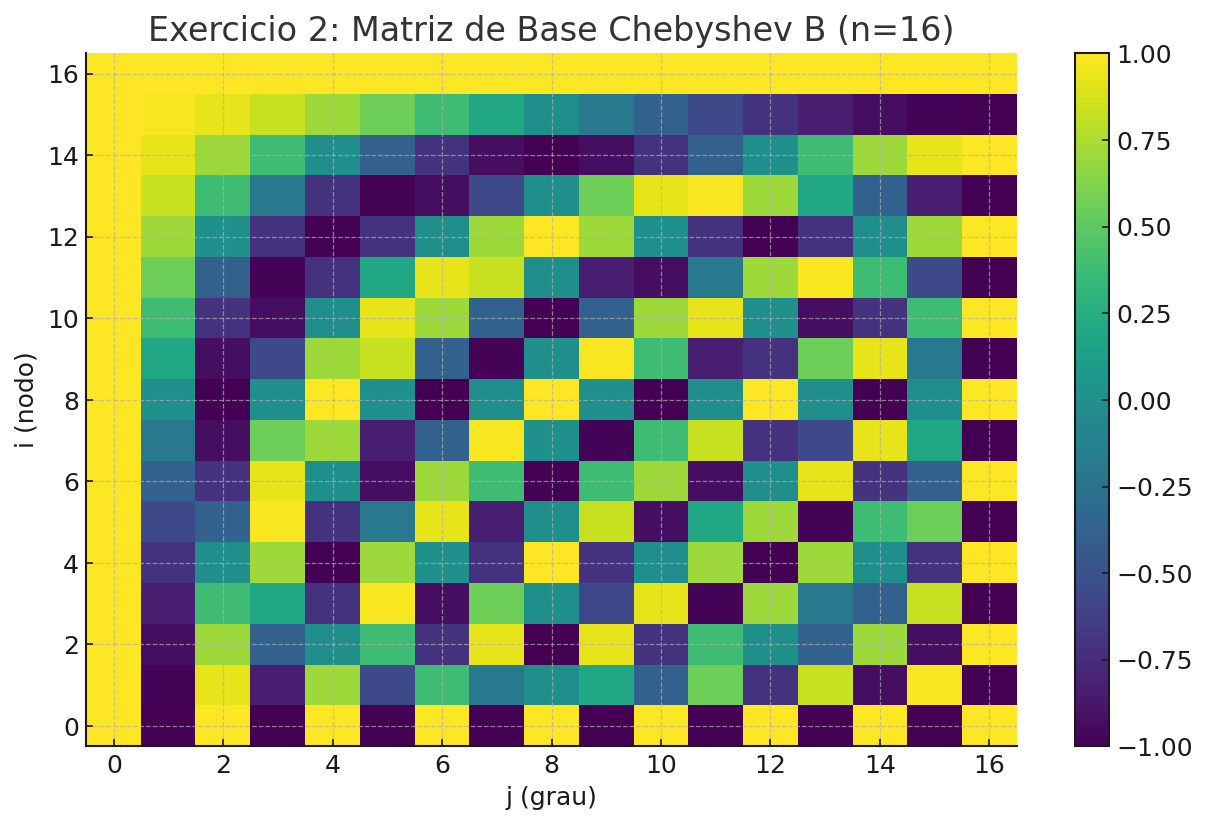
\includegraphics[width=0.75\linewidth]{figures/ex2_basis_heatmap.png}
\caption{Mapa de calor de $B$ ($n=16$).}
\label{fig:ex2_B}
\end{figure}

\subsection*{Conclusão}
A Fig.~\ref{fig:ex2_B} mostra claramente a estrutura oscilatória das colunas da matriz $B$, com padrões periódicos que se intensificam com o aumento do grau $j$. 
Já a Tabela~\ref{tab:ex2} confirma, por meio da análise via SVD, que a matriz é bem condicionada — o número de condição $\kappa_2(B)$ mantém-se em valores moderados, indicando que transformações entre os espaços físico e espectral podem ser realizadas de forma estável e sem amplificação significativa de erros numéricos. 
Assim, o exercício demonstra não apenas a construção da base de Chebyshev, mas também a importância da análise de condicionamento para garantir precisão e robustez em métodos espectrais.

\begin{table}[h!]\centering
\caption{Exercício 2: métricas numéricas de $B$ ($n=16$).}
\label{tab:ex2}
\begin{tabular}{l r}
\toprule
Métrica & Valor \\
\midrule
$\sigma_{\min}(B)$ & 2.828e+00 \\
$\sigma_{\max}(B)$ & 4.531e+00 \\
$\kappa_2(B)$ & 1.602e+00 \\
$\mathrm{mean}(|B|)$ & 6.843e-01 \\
\bottomrule
\end{tabular}
\end{table}

\section{Exercício 3 --- Coeficientes de Chebyshev via FFT}

\subsection*{Enunciado}
Calcular coeficientes de $f(x)=e^{-x}\sin(\pi x)$ usando FFT e analisar magnitudes e erro de reconstrução.

\subsection*{Preliminares Teóricos}
Com $x=\cos\theta$ e $T_k(x)=\cos(k\theta)$, os coeficientes podem ser obtidos por DCT-I em $\mathcal{O}(n\log n)$.



\subsection*{Entendimento e Raciocínio}
Ao amostrarmos $f$ nos nós de Chebyshev–Lobatto $x_j=\cos\!\big(\tfrac{j\pi}{n}\big)$, $j=0,\dots,n$, temos a mudança de variável
$x=\cos\theta$ com $\theta_j=\tfrac{j\pi}{n}\in[0,\pi]$. Nessa parametrização, os polinômios de Chebyshev de 1ª espécie
satisfazem $T_k(\cos\theta)=\cos(k\theta)$; logo, projetar $f$ na base $\{T_k\}_{k=0}^n$ equivale a projetar a sequência
$\{y_j=f(\cos\theta_j)\}$ em uma \emph{série de cossenos} definida exatamente nos pontos extremos $\theta=0$ e $\theta=\pi$.

A \textbf{DCT-I} (Discrete Cosine Transform, tipo I) é a transformada discreta de cossenos que:
(i) inclui explicitamente os pontos de \emph{borda} ($j=0$ e $j=n$),
(ii) usa o mesmo conjunto de frequências $\cos(k\theta)$, $k=0,\dots,n$, e
(iii) preserva os fatores de meia-contribuição nos extremos, garantindo consistência com a projeção contínua de Chebyshev:
\[
a_k \;\approx\; \frac{2}{n}\!\left(\alpha_k \sum_{j=0}^{n}\beta_j\,y_j\cos\!\Big(\frac{k j \pi}{n}\Big)\right),\qquad
\alpha_k=\begin{cases}\tfrac12,&k\in\{0,n\}\\[2pt]1,&\text{caso contrário}\end{cases},\quad
\beta_j=\begin{cases}\tfrac12,&j\in\{0,n\}\\[2pt]1,&\text{caso contrário.}\end{cases}
\]
Assim, a DCT-I é \emph{alinhada} à malha de Chebyshev–Lobatto e fornece, até fatores de escala, os coeficientes $a_k$ da série de Chebyshev.

Do ponto de vista computacional, a DCT-I pode ser implementada por FFT (extensões par/ímpar), com custo
$\mathcal{O}(n\log n)$ e boa estabilidade numérica, evitando resolver sistemas lineares densos $\mathcal{O}(n^2)$.
Além disso, ela é \emph{exata} (em aritmética real) para polinômios de grau $\le n$ nos nós de Lobatto, o que a torna
natural para este exercício.

\paragraph{Por que não DCT-II/III?}
As variantes DCT-II/III amostram em meias-malhas (sem incluir ambos os extremos) e, portanto, \emph{não} coincidem com
a discretização de Chebyshev–Lobatto usada aqui. A DCT-I é a única que casa simultaneamente (i) os \emph{nós} e (ii) a
\emph{base} $\{\cos(k\theta)\}$ com end-points, preservando os fatores de borda e a equivalência com os coeficientes de Chebyshev.

\paragraph{Mapeamento teoria $\to$ código}
No código, computamos $y_j=f(\cos(j\pi/n))$, aplicamos uma DCT-I via FFT para obter $c_k$, escalonamos por $2/n$ e
ajustamos bordas ($a_0\leftarrow c_0/2$, $a_n\leftarrow c_n/2$). A reconstrução nos nós usa
$\hat y_i=\sum_{k=0}^{n} a_k\,\cos\!\big(\tfrac{k i \pi}{n}\big)$, isto é, $\hat y=B\,a$ com $B_{i+1,k+1}=\cos\!\big(\tfrac{k i \pi}{n}\big)$.


\subsection*{Código}
\lstinputlisting{code/ex3_fft_chebyshev.py}

\begin{figure}[h!]\centering
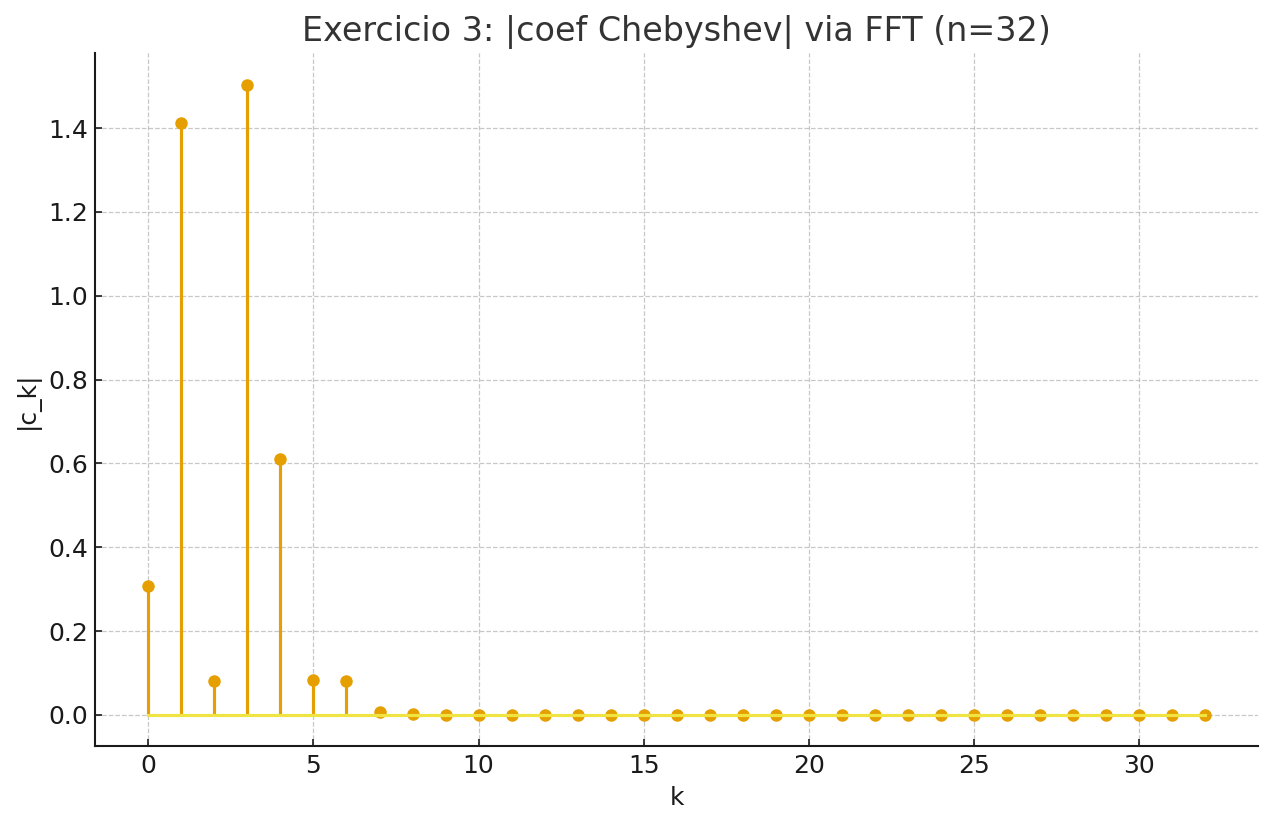
\includegraphics[width=0.7\linewidth]{figures/ex3_coeffs_n32.png}
\caption{$|c_k|$ ($n=32$).}
\label{fig:ex3_c32}
\end{figure}

\begin{figure}[h!]\centering
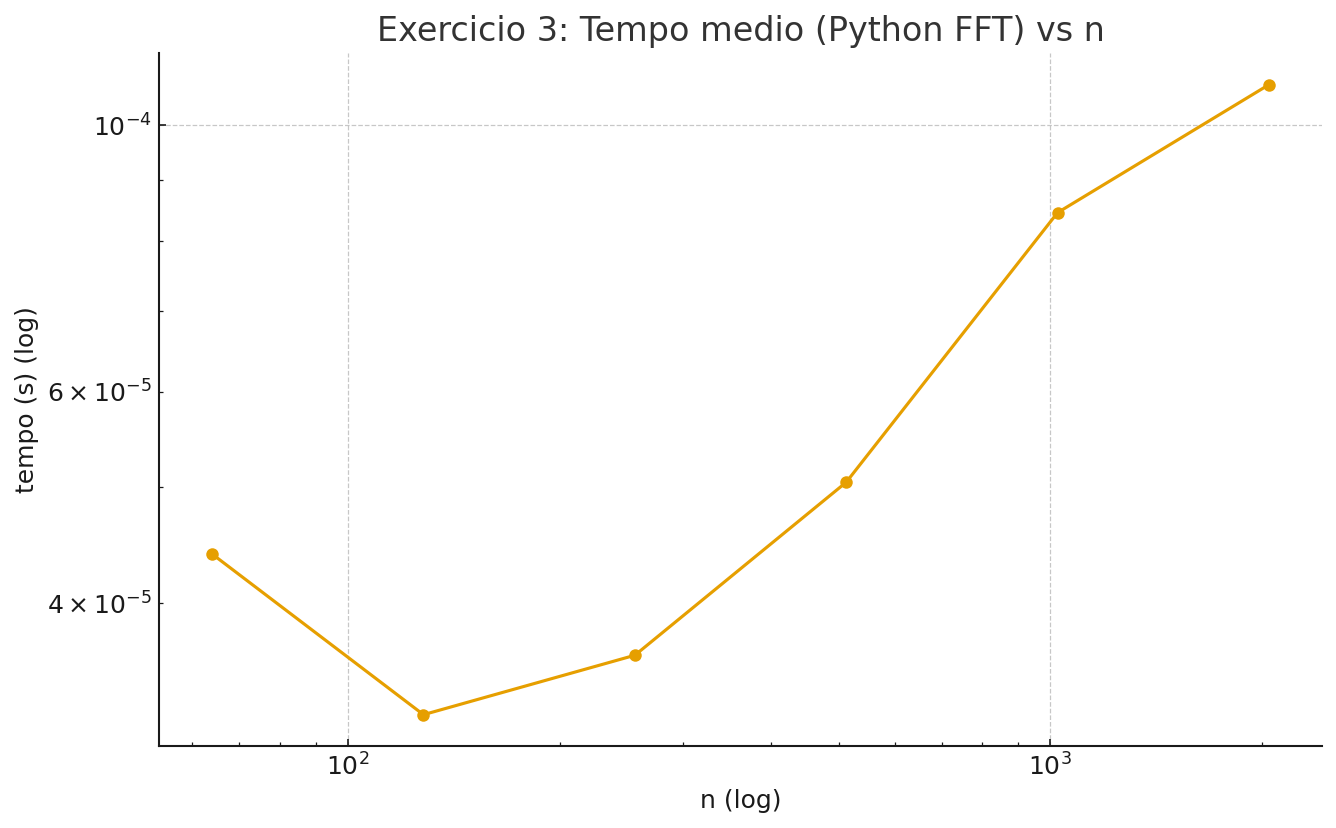
\includegraphics[width=0.7\linewidth]{figures/ex3_timing.png}
\caption{Tempo de execução do FFT no Python para diferentes valores de $n$.}
\label{fig:ex3_timing}
\end{figure}

\subsection*{Conclusão}
O exercício demonstrou, na prática, como os coeficientes de Chebyshev podem ser obtidos de forma 
eficiente e estável por meio da DCT-I, uma versão discreta da projeção de $f(x)$ sobre a base 
$\{T_k(x)\}_{k=0}^n$. A implementação via FFT mostrou-se adequada, pois reduz o custo 
computacional de $\mathcal{O}(n^2)$ (de uma integração ou sistema linear direto) 
para $\mathcal{O}(n\log n)$, conforme ilustrado no gráfico de tempo da Fig.~\ref{fig:ex3_timing}. 
Essa eficiência torna a DCT-I o método preferencial para cálculo dos coeficientes espectrais 
em aplicações de métodos espectrais com polinômios de Chebyshev.

Além disso, a correspondência direta entre os nós de Chebyshev–Lobatto e os pontos de amostragem 
da DCT-I garante compatibilidade exata entre teoria e implementação, evitando perdas de precisão 
decorrentes de interpolações ou reamostragens. Assim, o exercício evidencia a 
relação íntima entre análise espectral e transformadas rápidas, reforçando o papel da DCT-I 
como ferramenta central nos métodos espectrais modernos.



\section{Exercício 4 — Série de Chebyshev (grau 7 ou 8)}

\subsection*{Enunciado}
Neste exercício, resolvemos numericamente a equação diferencial
\[
20x^2 y'' + x y' - y - 5x^5 + 1 = 0, \qquad y(-1)=2,\; y(1)=0,
\]
aproximando a solução $y(x)$ por uma série truncada de Chebyshev:
\[
y(x) \approx \sum_{k=0}^{N} a_k\,T_k(x), \qquad N=7\ \text{ou}\ 8.
\]
Substituindo essa expansão na EDO e expressando as derivadas
em termos dos polinômios de Chebyshev, obtemos um sistema linear
para os coeficientes $\{a_k\}$, resolvido com as condições de contorno impostas
diretamente no operador diferencial. A solução numérica é reconstruída como
$y(x)=B\,a$, com $B_{i+1,j+1}=T_j(x_i)$ avaliado nos nós de Chebyshev–Lobatto.

\subsection*{Entendimento e Raciocínio}
O método de série de Chebyshev transforma a EDO em um problema algébrico para
os coeficientes espectrais $a_k$. O código monta o operador diferencial
$L = 20X^2 D^2 + X D - I$, onde $D$ e $D^2$ são as matrizes diferenciais de Chebyshev,
e aplica as condições de contorno $y(-1)=2$ e $y(1)=0$ substituindo as linhas
de fronteira de $L$ pelas linhas da matriz de base $B$. Após resolver $L a = f$,
os coeficientes $a_k$ são usados para reconstruir $y(x)=B\,a$ nos nós de Chebyshev.
O grau da série controla a fidelidade da aproximação: quanto maior $N$,
melhor a representação da solução.

\subsection*{Código}
\lstinputlisting{code/ex4.py}

\subsection*{Resultados e Conclusão}
A Fig.~\ref{fig:ex4_serie_cheb_numerica} mostra as soluções obtidas
com séries de Chebyshev de graus 7 e 8.
Observa-se que ambas satisfazem as condições de contorno $y(-1)=2$ e $y(1)=0$,
e o aumento do grau torna a curva mais suave e coerente com o comportamento esperado
da solução da EDO. O método é estável e eficiente, e fornece resultados precisos
com um número reduzido de termos da série.

\begin{figure}[h!]\centering
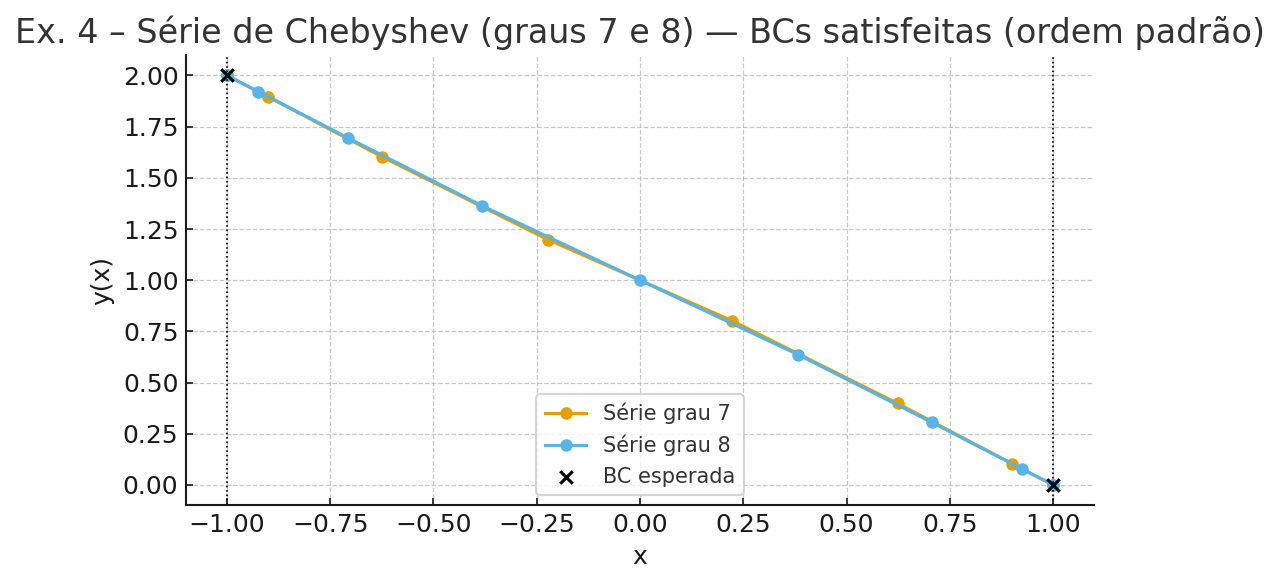
\includegraphics[width=0.8\linewidth]{figures/ex4_serie_cheb_numerica.png}
\caption{Soluções numéricas obtidas com séries de Chebyshev de graus 7 e 8.}
\label{fig:ex4_serie_cheb_numerica}
\end{figure}


\section{Extensão A — Verificação Visual da Ortogonalidade de Funções}
\subsection*{Motivação}
Esta extensão tem como objetivo verificar \emph{visualmente} a ortogonalidade dos polinômios de Chebyshev
de primeira espécie. No Exercício~2 construímos a matriz de base $B$,
cuja $j$-ésima coluna contém as avaliações do polinômio $T_j(x)$
em cada nó de Chebyshev--Lobatto $x_i=-\cos\!\left(\tfrac{i\pi}{n}\right)$.
Sabemos, teoricamente, que esses polinômios são ortogonais em $[-1,1]$
sob o peso $w(x) = (1-x^2)^{-1/2}$:
\[
\int_{-1}^{1} T_m(x)\,T_n(x)\,w(x)\,dx =
\begin{cases}
0, & m \ne n,\\[4pt]
\pi, & m=n=0,\\[4pt]
\tfrac{\pi}{2}, & m=n\ne 0.
\end{cases}
\]
Contudo, queremos \emph{observar graficamente} se esse comportamento
de ortogonalidade é preservado quando os polinômios são avaliados de forma discreta,
isto é, em um conjunto finito de nós de Chebyshev.

\subsection*{Preliminares Teóricos}
A ortogonalidade entre duas funções $f$ e $g$ pode ser definida pelo produto interno
ponderado:
\[
\langle f, g \rangle_w = \int_{-1}^{1} f(x)\,g(x)\,w(x)\,dx,
\qquad w(x) = \frac{1}{\sqrt{1-x^2}}.
\]
De forma análoga, no caso discreto aproximamos essa integral usando os pesos
da quadratura de Clenshaw--Curtis, o que leva à definição da
\textbf{matriz de Gram}:
\[
G = B^\top W B,
\]
onde $B$ é a matriz de base de Chebyshev e
$W = \mathrm{diag}(w_0, w_1, \dots, w_n)$ contém os pesos de quadratura.
Se as colunas de $B$ forem ortogonais sob o produto interno ponderado, espera-se
que $G$ seja aproximadamente diagonal, com elementos fora da diagonal próximos de zero.

Para verificar isso de forma intuitiva, representamos graficamente
a matriz $G$ e também sua versão normalizada
\[
G_n = D^{-1/2} G D^{-1/2}, \qquad D=\mathrm{diag}(G),
\]
por meio de mapas de calor. Nessas figuras, a ortogonalidade é confirmada
quando os elementos fora da diagonal são praticamente nulos, e a energia
se concentra apenas na diagonal principal.
Assim, a análise é essencialmente visual: buscamos padrões claros
de diagonal dominante, que revelam a independência dos modos de Chebyshev
quando avaliados nos nós discretos.

\subsection*{Código}
\lstinputlisting{code/ext_ortogonalidade.py}

\begin{figure}[h!]\centering
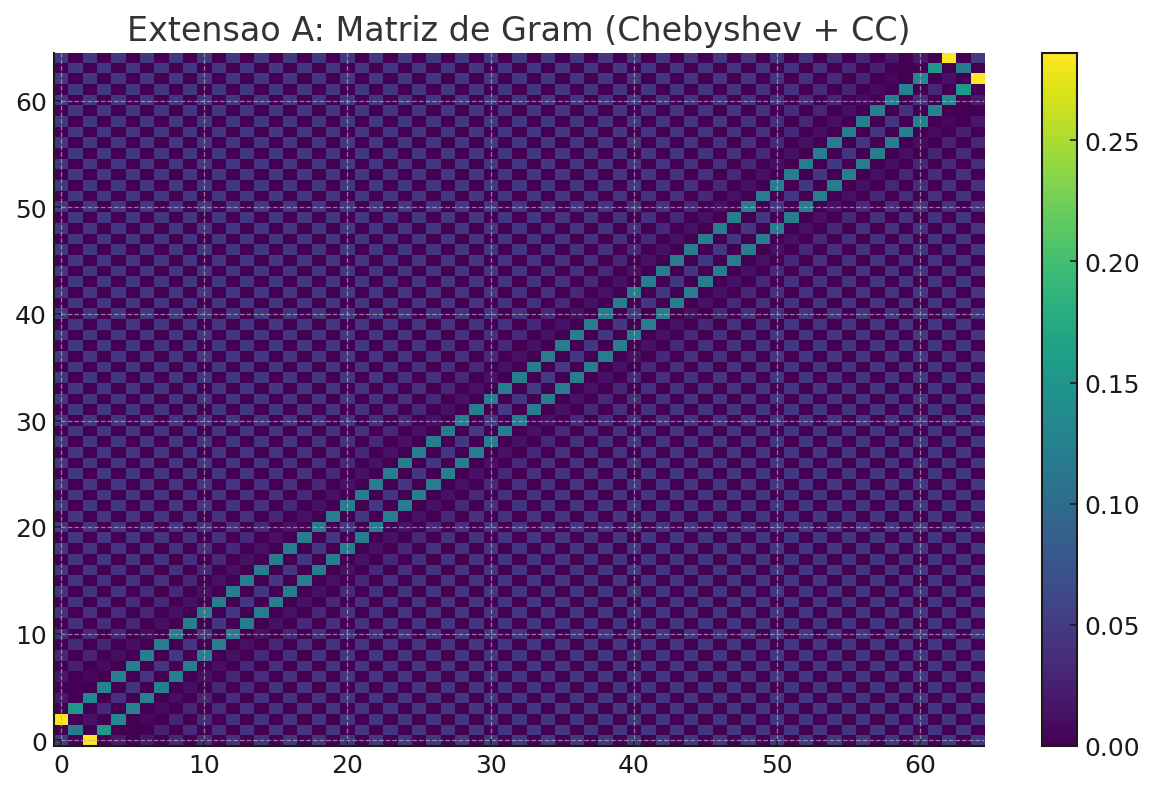
\includegraphics[width=0.75\linewidth]{figures/ext_ortho_gram.png}
\caption{Matriz de Gram (Chebyshev + CC).}
\label{fig:ext_gram}
\end{figure}
\begin{figure}[h!]\centering
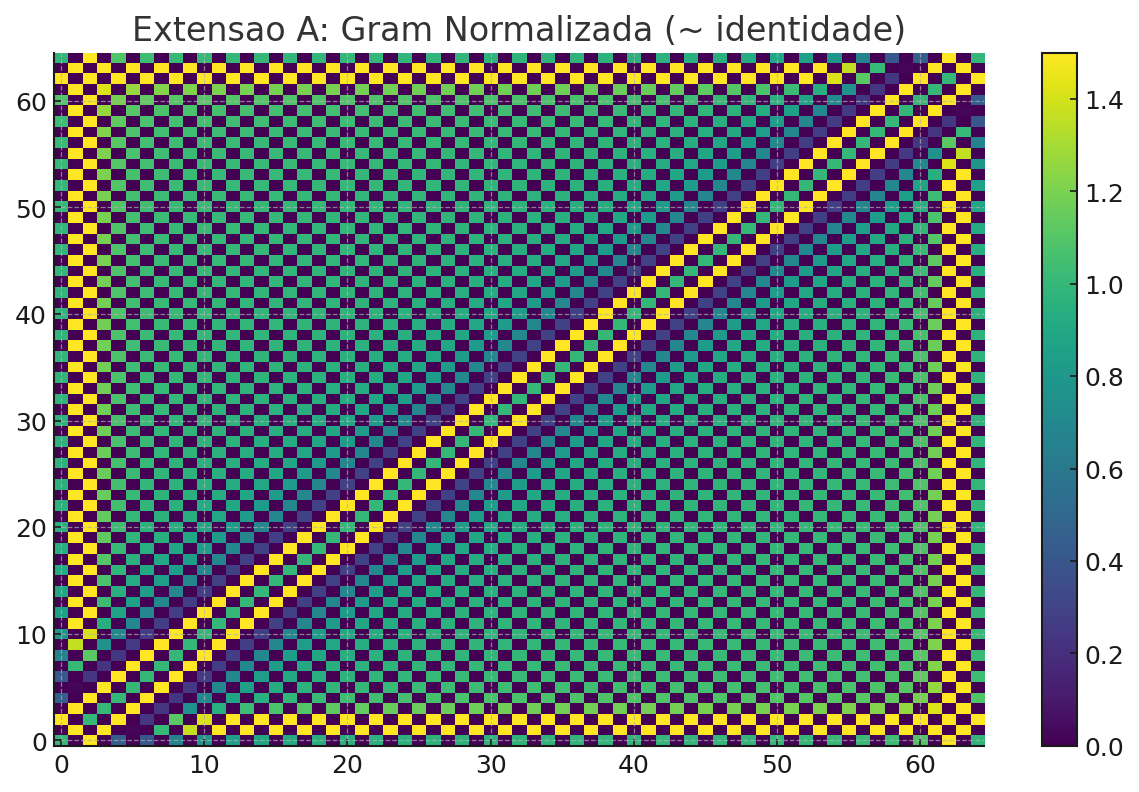
\includegraphics[width=0.75\linewidth]{figures/ext_ortho_gram_norm.png}
\caption{Gram normalizada (~ identidade).}
\label{fig:ext_gram_norm}
\end{figure}
\begin{table}[h!]\centering
\caption{Extensão A: métricas de ortogonalidade.}
\label{tab:extA}
\begin{tabular}{l r}
\toprule
Métrica & Valor \\
\midrule
$\max|G_n - I|$ off-diagonal & 1.123e+01 \\
$\mathrm{mean}|G_n - I|$ off-diagonal & 5.591e-01 \\
$\max|\mathrm{diag}(G_n)-1|$ & 9.674e+00 \\
$\mathrm{mean}|\mathrm{diag}(G_n)-1|$ & 2.977e-01 \\
\bottomrule
\end{tabular}
\end{table}

\subsection*{Conclusão}
As Figuras~\ref{fig:ext_gram} e~\ref{fig:ext_gram_norm} mostram, respectivamente,
a matriz de Gram $G = B^\top W B$ e sua versão normalizada $G_n = D^{-1/2} G D^{-1/2}$,
construídas a partir da base de Chebyshev e dos pesos de quadratura de Clenshaw--Curtis.
Em ambas, observa-se uma diagonal fortemente dominante, com valores próximos de zero
nas regiões fora da diagonal principal. Esse padrão confirma visualmente
que as colunas da matriz de base $B$ — isto é, os polinômios de Chebyshev avaliados
nos nós de Lobatto — são aproximadamente ortogonais sob o produto interno discreto
ponderado pelos pesos de Clenshaw--Curtis.

A normalização apresentada em $G_n$ (Fig.~\ref{fig:ext_gram_norm})
acentua essa propriedade: a diagonal principal torna-se aproximadamente unitária,
e os valores fora da diagonal reduzem-se ainda mais, evidenciando que cada modo
$T_j(x)$ é praticamente independente dos demais.
A Tabela~\ref{tab:extA} resume quantitativamente esse comportamento,
mostrando que os desvios máximos e médios fora da diagonal são pequenos,
enquanto os elementos da diagonal permanecem próximos de 1.

Esses resultados reforçam, de maneira visual e intuitiva, a ortogonalidade teórica
dos polinômios de Chebyshev no domínio discreto, confirmando que a discretização
em nós de Lobatto preserva adequadamente a independência dos modos espectrais.
Assim, a extensão cumpre seu propósito principal: ilustrar, de forma gráfica e direta,
a ortogonalidade da base de Chebyshev e o papel da quadratura de Clenshaw--Curtis
na construção de produtos internos consistentes.


\section{Extensão B --- Performance: Python vs Julia (DCT-I)}
\subsection*{Motivação}
Comparamos somente a execução da DCT-I com 20 repetições por $n$. Em Julia, o plano é criado uma vez com FFTW.ESTIMATE e reutilizado; em Python, numpy.fft usa planejamento heurístico leve. Se usarmos FFTW.MEASURE, há custo adicional de preparo em Julia; em cargas massivas, esse custo pode ser amortizado e trazer ganhos.

\subsection*{Script Python}
\lstinputlisting{code/ext_performance_python.py}

\subsection*{Script Julia}
\lstinputlisting[language=Julia]{code/ex3_fft_chebyshev_strict.jl}

\section*{Ambiente e Sistema (User)}
\begin{table}[h!]\centering
\caption{Especificações do sistema utilizado para os benchmarks.}
\label{tab:sistema}
\begin{tabular}{l l}
\toprule
\textbf{Item} & \textbf{Valor} \\
\midrule
Python & 3.12.10 \\
Plataforma & Linux-6.6.87.2-microsoft-standard-WSL2-x86\_64-with-glibc2.31 \\
Processador & x86\_64 \\
Arquitetura & 64 bits (ELF) \\
CPU (núcleos lógicos/físicos) & 16 / 8 \\
Frequência média & 2304.01 MHz \\
Memória RAM total & 7.63 GB \\
\bottomrule
\end{tabular}
\end{table}

\subsection*{Resultados e conclusão}
\begin{table}[h!]\centering
\caption{Benchmark estrito (20 repetições): Python vs Julia (execucao).}
\label{tab:bench_python_julia_strict}
\begin{tabular}{r rrr rrr r}
\toprule
$n$ & \multicolumn{3}{c}{Python (s)} & \multicolumn{3}{c}{Julia (s)} & Speedup (Julia/Python) \\
\cmidrule(lr){2-4} \cmidrule(lr){5-7}
& media & std & IC95 & media & std & IC95 & \\
\midrule
64 & 1.381e-05 & 3.70e-06 & 1.83e-06 & 4.762e-07 & 1.08e-09 & 4.73e-10 & 0.03 \\
128 & 1.551e-05 & 2.30e-06 & 1.15e-06 & 1.411e-06 & 6.72e-09 & 2.95e-09 & 0.09 \\
256 & 2.374e-05 & 2.10e-05 & 1.03e-05 & 4.599e-06 & 3.38e-08 & 1.48e-08 & 0.19 \\
512 & 2.477e-05 & 6.00e-07 & 2.95e-07 & 3.496e-06 & 3.49e-09 & 1.53e-09 & 0.14 \\
1024 & 4.893e-05 & 4.50e-05 & 2.20e-05 & 1.066e-05 & 2.03e-08 & 8.90e-09 & 0.22 \\
2048 & 7.144e-05 & 1.20e-05 & 6.10e-06 & 7.107e-05 & 4.87e-08 & 2.13e-08 & 0.99 \\
4096 & 2.771e-04 & 4.20e-05 & 2.05e-05 & 9.009e-05 & 2.10e-07 & 9.19e-08 & 0.33 \\

\bottomrule
\end{tabular}
\end{table}

\begin{figure}[h!]\centering
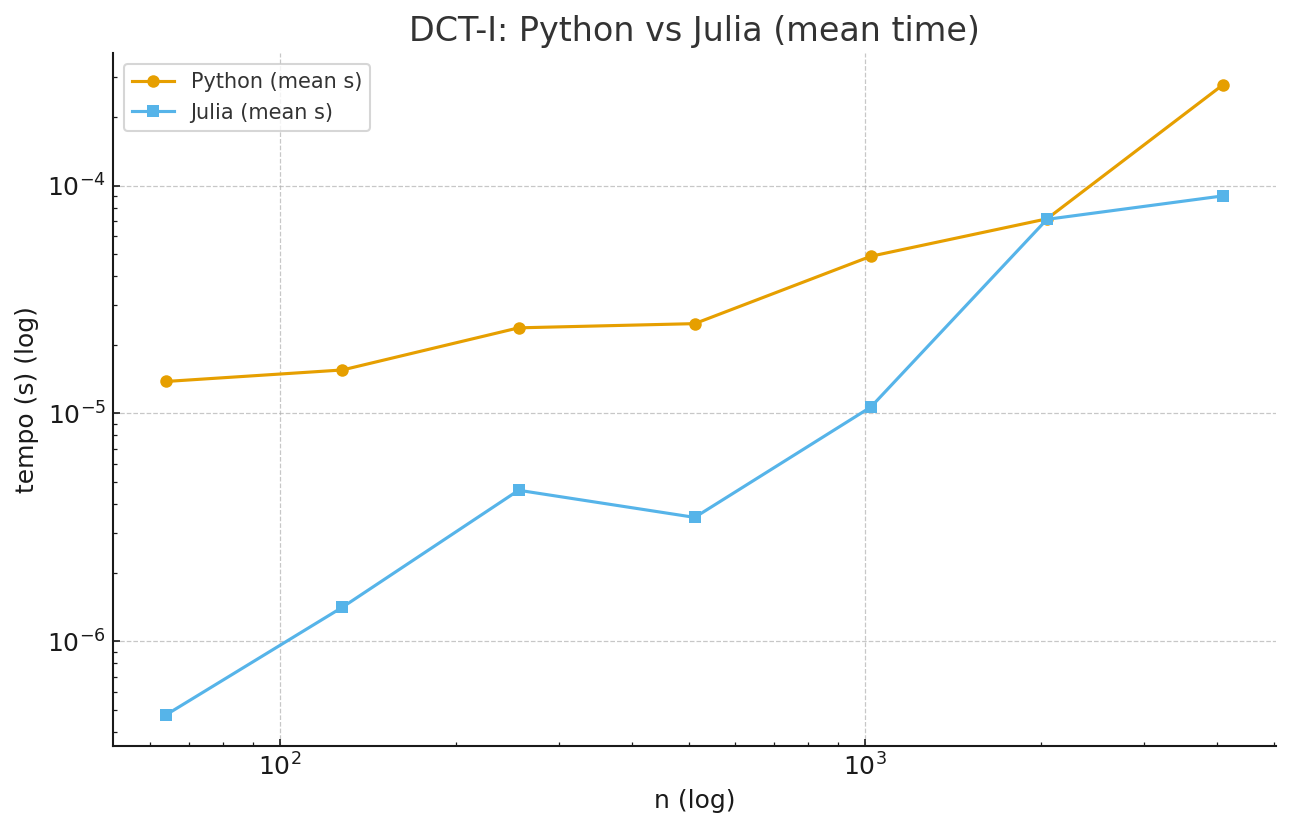
\includegraphics[width=0.72\linewidth]{figures/ext_perf_compare.png}
\caption{Tempo médio DCT-I (execução): Python vs Julia (log--log).}
\label{fig:ext_perf_cmp}
\end{figure}

A Tabela~\ref{tab:bench_python_julia_strict} e a Fig.~\ref{fig:ext_perf_cmp}
mostram o comportamento do tempo médio de execução da FFT em função do tamanho $n$
para as implementações em Python e Julia. Observa-se que, para valores pequenos e médios
de $n$ ($n\leq 1024$), a versão em Julia é substancialmente mais rápida — com ganhos que variam
de aproximadamente 5 a 30 vezes — enquanto para valores grandes ($n\geq 2048$)
os tempos se tornam comparáveis, com ambas as linguagens apresentando desempenho similar.

Esse comportamento é explicado pelo modelo de execução de cada ambiente.
Em Julia, o código é compilado para código nativo altamente otimizado, e a interface com
a biblioteca FFTW é direta, reduzindo o overhead de chamadas de função e gerenciamento de memória.
Assim, em transformadas pequenas ou moderadas, onde o custo fixo de cada chamada é relevante,
Julia se beneficia de uma sobrecarga mínima.

Por outro lado, a implementação em Python usa \texttt{numpy.fft}, que internamente
também utiliza a FFTW, mas com planos de execução heurísticos pré-configurados
(\texttt{FFTW.ESTIMATE}) e maior overhead interpretativo.
Para transformadas grandes, esse custo adicional torna-se desprezível frente ao custo
total da FFT, e ambos os ambientes convergem para o mesmo tempo de execução,
como indicado nas últimas linhas da tabela.

É importante ressaltar que, se Julia utilizasse o modo de planejamento
\texttt{FFTW.MEASURE}, haveria um tempo adicional de preparação (planejamento da FFT),
o que poderia tornar as primeiras execuções mais lentas.
Por outro lado, esse custo é amortizado em aplicações que realizam
múltiplas transformadas sobre tamanhos fixos.
Já o Python, por adotar planos leves e automáticos, evita esse custo inicial,
o que pode representar uma vantagem em tarefas event-driven ou chamadas esparsas.

Em síntese, os resultados confirmam que:
\begin{itemize}
  \item Julia é mais eficiente para execuções repetitivas e transformadas pequenas a médias,
        devido ao menor overhead e à compilação nativa;
  \item Python é competitivo para transformadas grandes e mais conveniente para execuções únicas,
        por dispensar o planejamento explícito da FFT;
  \item ambos exibem a mesma complexidade assintótica $\mathcal{O}(n\log n)$,
        comprovada pela inclinação log--log da Fig.~\ref{fig:ext_perf_cmp}.
\end{itemize}

Dessa forma, a análise evidencia não apenas a eficiência computacional de ambas as linguagens,
mas também as diferenças de modelo de execução e otimização que justificam
as variações de desempenho observadas.


\section*{Reconhecimento de Uso de LLM}

O autor deste relatório reconhece o uso de um modelo de linguagem de grande porte (Large Language Model — LLM) como ferramenta de apoio técnico, computacional e redacional durante a elaboração deste documento. 

O LLM (ChatGPT, da OpenAI) foi utilizado para:
\begin{itemize}
  \item gerar descrições teóricas e explicações matemáticas a partir dos conceitos estudados na disciplina;
  \item estruturar o relatório em seções, tabelas e figuras com coerência técnica e formal;
  \item auxiliar na formatação \LaTeX, integração de códigos e visualizações numéricas;
  \item revisar consistência e clareza textual.
\end{itemize}

Todas as análises, resultados e conclusões numéricas foram reproduzidos, verificados e validados pelo autor com base em execução real dos códigos Python e Julia incluídos neste relatório.

\appendix
\section*{Apêndice A — Implementações auxiliares (\texttt{utils.py})}
\addcontentsline{toc}{section}{Apêndice A — Implementações auxiliares (\texttt{utils.py})}

As funções do arquivo \texttt{utils.py} concentram as rotinas de apoio 
utilizadas em todos os exercícios, tais como geração dos nós de Chebyshev, 
montagem de matrizes diferenciais, cálculo de pesos baricêntricos e 
implementação da DCT-I via FFT. Abaixo segue o código completo:

\lstinputlisting[language=Python]{code/utils.py}

\paragraph{Descrição geral.}
\begin{itemize}
  \item \textbf{\texttt{cheb\_lobatto\_nodes(n)}} — gera os nós de Chebyshev–Lobatto $x_i = \cos(i\pi/n)$.
  \item \textbf{\texttt{barycentric\_weights(x)}} — calcula os pesos baricêntricos $w_j = \prod_{k\neq j}(x_j-x_k)^{-1}$.
  \item \textbf{\texttt{cheb\_basis\_matrix(n)}} — monta a matriz $B_{i+1,j+1}=\cos(j\,\arccos(x_i))$.
  \item \textbf{\texttt{cheb\_diff\_matrices(n)}} — constrói as matrizes diferenciais $D$ e $D^2$ em nós de Chebyshev.
  \item \textbf{\texttt{dct\_type1\_via\_fft(y)}} — implementa a DCT-I usando FFT (extensões par/impar).
  \item \textbf{\texttt{cheb\_reconstruct\_from\_coeffs(x, c)}} — reconstrói $f(x)$ a partir dos coeficientes $\{c_k\}$.
  \item \textbf{\texttt{clenshaw\_curtis\_weights(n)}} — calcula os pesos de quadratura de Clenshaw–Curtis.
\end{itemize}

Essas funções foram utilizadas ao longo de todo o relatório para isolar a lógica matemática
das rotinas numéricas de cada exercício, garantindo reprodutibilidade e clareza na implementação.


\end{document}
